% IEEEtran skeleton: section headings only, with figures and tables placed.
% Compile: tectonic main.tex   (or pdflatex/bibtex from report_assets/)
\documentclass[conference]{IEEEtran}
\usepackage{graphicx}
\usepackage{booktabs}
\usepackage{array}
\usepackage{amsmath,amssymb}
\usepackage{newtxtext,newtxmath}
\usepackage[hidelinks]{hyperref}
\graphicspath{{figures/}{diagrams/}}

\begin{document}

\title{Amortized Post-Quantum Secure Aggregation for Federated Learning}
\author{\IEEEauthorblockN{Author Name}
\IEEEauthorblockA{Affiliation\\ email}}
\maketitle

\begin{abstract}
\end{abstract}

\begin{IEEEkeywords}
post-quantum cryptography, federated learning, ML-KEM, ML-DSA, secure aggregation
\end{IEEEkeywords}

\section{Introduction}

\section{Background}
\subsection{Post-Quantum KEMs and Signatures}
\subsection{Federated Learning and Update Confidentiality}

\section{Threat Model}

\section{Protocol Design}
\label{sec:design}

\begin{figure*}[t]
  \centering
  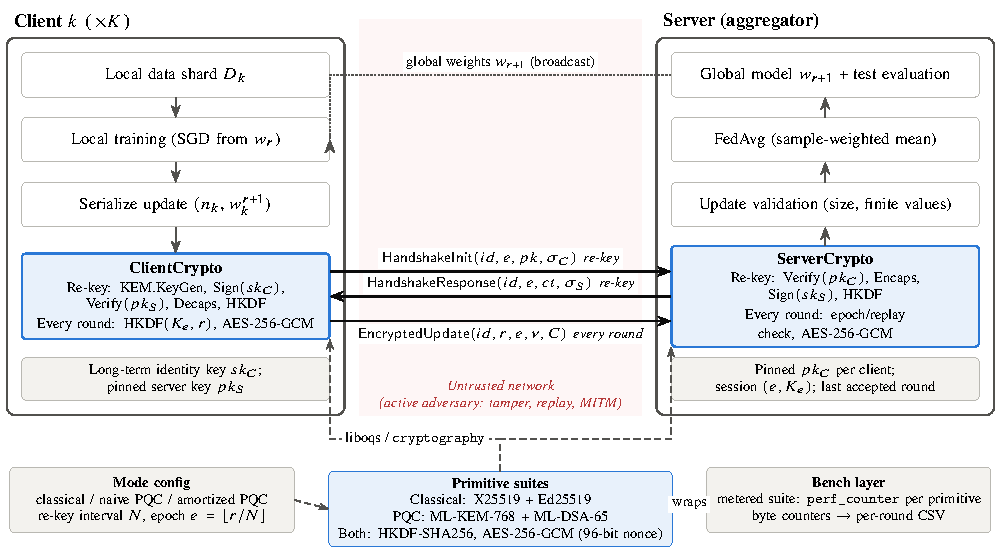
\includegraphics[width=\textwidth]{architecture.pdf}
  \caption{System architecture.}
  \label{fig:architecture}
\end{figure*}

\subsection{Session Setup}
\subsection{Per-Round Update Encryption}
\subsection{Re-Keying Schedule}

\begin{figure*}[t]
  \centering
  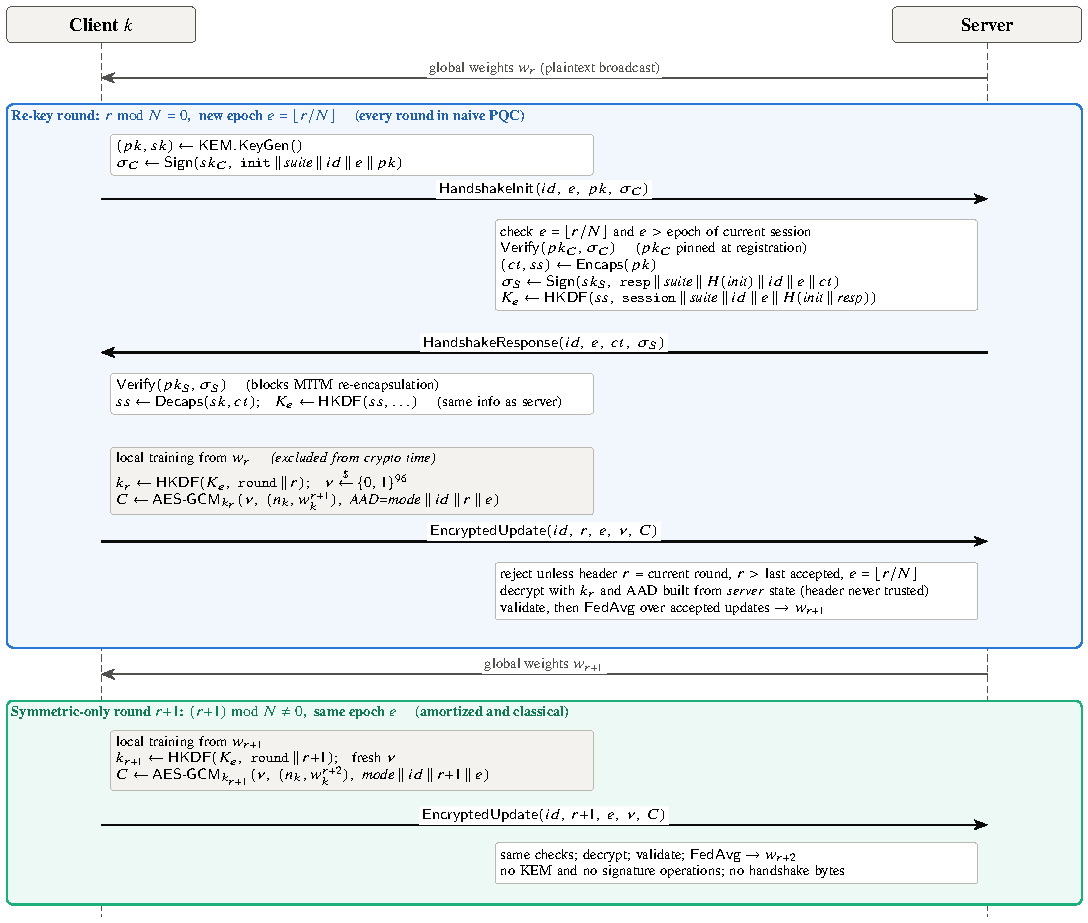
\includegraphics[width=0.92\textwidth]{sequence.pdf}
  \caption{Message sequence for a re-key round followed by a symmetric-only round.}
  \label{fig:sequence}
\end{figure*}

\subsection{Operating Modes}

\section{Implementation}

\section{Experimental Setup}

\section{Results}
\label{sec:results}

% Generated by scripts/make_report_assets.py -- do not edit by hand.
\begin{table*}[t]
\centering
\footnotesize
\caption{Main comparison of the three modes}
\label{tab:main}
\setlength{\tabcolsep}{4pt}
\begin{tabular}{lrrrrrrrr}
\toprule
Mode & $N$ & HS & Crypto (ms) & Handshake (ms) & AES-GCM (ms) & HS KB/client & \% round & Acc. (\%) \\
\midrule
Classical & 5 & 20 & 38.00 $\pm$ 0.61 & 9.10 $\pm$ 0.08 & 28.89 $\pm$ 0.55 & 0.8 & 0.089 $\pm$ 0.001 & 98.21 $\pm$ 0.06 \\
Naive PQC & 1 & 100 & 79.87 $\pm$ 0.54 & 50.66 $\pm$ 0.84 & 29.21 $\pm$ 0.43 & 173.6 & 0.182 $\pm$ 0.003 & 98.21 $\pm$ 0.06 \\
Amortized PQC & 5 & 20 & 39.93 $\pm$ 0.60 & 10.25 $\pm$ 0.17 & 29.68 $\pm$ 0.46 & 34.7 & 0.091 $\pm$ 0.001 & 98.21 $\pm$ 0.06 \\
\bottomrule
\end{tabular}
\\[2pt]\parbox{\linewidth}{\scriptsize $K=5$, 20 rounds, 5 seeds; times summed over all clients and the server; HS = handshakes; \% round = crypto share of wall-clock round time incl.\ local training, excl.\ test-set evaluation.}
\end{table*}


\subsection{Per-Round and Cumulative Crypto Overhead}

\begin{figure}[t]
  \centering
  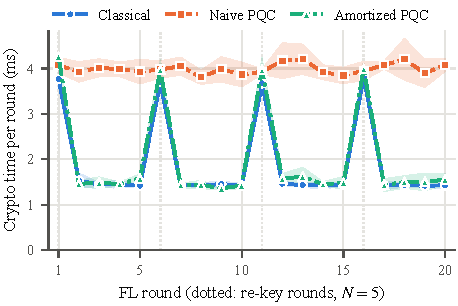
\includegraphics[width=\columnwidth]{crypto_per_round.pdf}
  \caption{Crypto time per round by mode (mean $\pm$ std over seeds).}
  \label{fig:per_round}
\end{figure}

\begin{figure}[t]
  \centering
  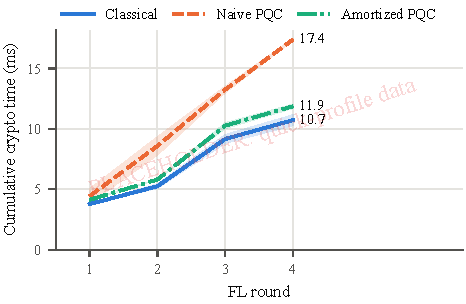
\includegraphics[width=\columnwidth]{crypto_cumulative.pdf}
  \caption{Cumulative crypto time over rounds by mode.}
  \label{fig:cumulative}
\end{figure}

% Generated by scripts/make_report_assets.py -- do not edit by hand.
\begin{table}[t]
\centering
\footnotesize
\caption{Time per primitive over a session (ms)}
\label{tab:primitives}
\setlength{\tabcolsep}{4pt}
\begin{tabular}{lrrrrr}
\toprule
Mode & KeyGen & Encaps & Decaps & Sign & Verify \\
\midrule
Classical & 0.978 $\pm$ 0.019 & 1.126 $\pm$ 0.008 & 0.989 $\pm$ 0.005 & 2.086 $\pm$ 0.007 & 2.924 $\pm$ 0.007 \\
Naive PQC & 5.231 $\pm$ 0.103 & 2.167 $\pm$ 0.023 & 2.225 $\pm$ 0.013 & 23.938 $\pm$ 0.927 & 10.634 $\pm$ 0.045 \\
Amortized PQC & 1.140 $\pm$ 0.025 & 0.455 $\pm$ 0.008 & 0.449 $\pm$ 0.002 & 4.749 $\pm$ 0.133 & 2.147 $\pm$ 0.010 \\
\bottomrule
\end{tabular}
\\[2pt]\parbox{\linewidth}{\scriptsize KEM keygen only; long-term identity keys are generated once at setup.}
\end{table}


\subsection{Communication Overhead}

% Generated by scripts/make_report_assets.py -- do not edit by hand.
\begin{table*}[t]
\centering
\footnotesize
\caption{Compute versus bandwidth overhead per round}
\label{tab:overhead}
\setlength{\tabcolsep}{4pt}
\begin{tabular}{lrrrrr}
\toprule
Mode & Crypto/round (ms) & Crypto \% of round & Wire KB/client/round & Overhead B/client/round & Overhead \% of payload \\
\midrule
Classical & 1.900 $\pm$ 0.031 & 0.089 $\pm$ 0.001 & 841.4 & 123 & 0.014 \\
Naive PQC & 3.994 $\pm$ 0.027 & 0.182 $\pm$ 0.003 & 850.1 & 9{,}026 & 1.048 \\
Amortized PQC & 1.997 $\pm$ 0.030 & 0.091 $\pm$ 0.001 & 843.1 & 1{,}863 & 0.216 \\
\bottomrule
\end{tabular}
\\[2pt]\parbox{\linewidth}{\scriptsize $K=5$, $N=5$ (Naive PQC: $N=1$), 20 rounds, 5 seeds. Round time is wall-clock including local training, excluding test-set evaluation. Overhead bytes = all protocol bytes beyond the serialized update (KEM keys and ciphertexts, signatures, nonce, GCM tag, framing).}
\end{table*}


\begin{figure}[t]
  \centering
  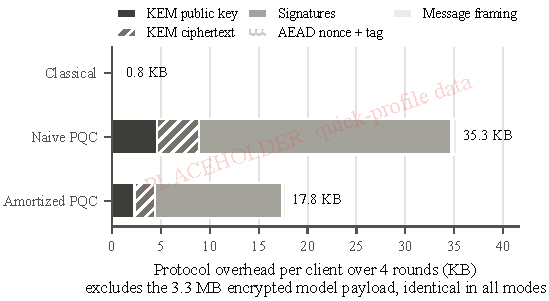
\includegraphics[width=\columnwidth]{bytes_components.pdf}
  \caption{Protocol bytes on the wire per client, by component.}
  \label{fig:bytes}
\end{figure}

\begin{figure}[t]
  \centering
  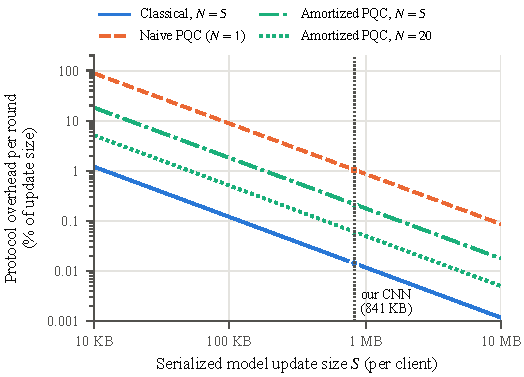
\includegraphics[width=\columnwidth]{bandwidth_vs_model_size.pdf}
  \caption{Per-round protocol overhead versus model update size $S$, computed as
  $100\,(o + H/N)/S$\,\% from measured byte counts: $o$ bytes per update (nonce, GCM tag,
  framing) and $H$ bytes per handshake per client. Markers: our CNN.}
  \label{fig:bandwidth}
\end{figure}

% Generated by scripts/make_report_assets.py -- do not edit by hand.
\begin{table*}[t]
\centering
\footnotesize
\caption{Per-round protocol overhead (\% of model update) versus update size}
\label{tab:bandwidth}
\setlength{\tabcolsep}{4pt}
\begin{tabular}{lrrrr}
\toprule
Update size $S$ & Classical{,} $N=5$ & Naive PQC ($N=1$) & Amortized PQC{,} $N=5$ & Amortized PQC{,} $N=20$ \\
\midrule
10 KB & 1.2 & 88.1 & 18.2 & 5.08 \\
100 KB & 0.12 & 8.81 & 1.82 & 0.508 \\
\textbf{841 KB (our CNN)} & 0.0143 & 1.05 & 0.216 & 0.0603 \\
1 MB & 0.0117 & 0.861 & 0.178 & 0.0496 \\
10 MB & 0.00117 & 0.0861 & 0.0178 & 0.00496 \\
\bottomrule
\end{tabular}
\\[2pt]\parbox{\linewidth}{\scriptsize Overhead $= 100\,(o + H/N)/S$\,\% per client per round, with measured $o=72$\,B per update (nonce, GCM tag, framing), $H=256$\,B per classical handshake and $H=8{,}954$\,B per PQC handshake (KEM key and ciphertext, two signatures, framing). Steady state ($R$ a multiple of $N$).}
\end{table*}


\subsection{Effect of Re-Key Interval}

\begin{figure}[t]
  \centering
  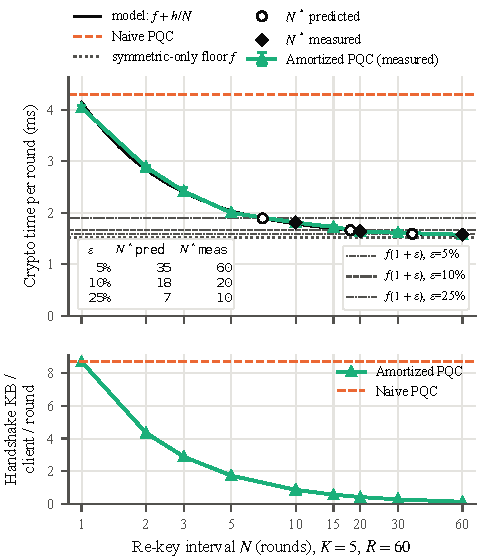
\includegraphics[width=\columnwidth]{rekey_sweep.pdf}
  \caption{Overhead versus re-key interval $N$ (amortized PQC) with the cost model $f + h/N$.
  $N^*(\varepsilon)$: smallest $N$ whose handshake overhead per round is at most $\varepsilon f$,
  predicted as $\lceil h/(\varepsilon f)\rceil$ and measured, for $\varepsilon \in \{5, 10, 25\}\%$.}
  \label{fig:rekey}
\end{figure}

% Generated by scripts/make_report_assets.py -- do not edit by hand.
\begin{table}[t]
\centering
\footnotesize
\caption{Amortized PQC versus re-key interval $N$ (times in ms)}
\label{tab:rekey}
\setlength{\tabcolsep}{3.5pt}
\begin{tabular}{lrrrrr}
\toprule
$N$ & HS rounds & Crypto/round & HS overhead/round & Model $h/N$ & \% of $f$ \\
\midrule
1 & 60 & 4.041 $\pm$ 0.046 & 2.563 $\pm$ 0.039 & 2.638 & 169.1 \\
2 & 30 & 2.888 $\pm$ 0.024 & 1.358 $\pm$ 0.012 & 1.319 & 89.6 \\
3 & 20 & 2.416 $\pm$ 0.073 & 0.892 $\pm$ 0.029 & 0.879 & 58.9 \\
5 & 12 & 2.001 $\pm$ 0.020 & 0.529 $\pm$ 0.010 & 0.528 & 34.9 \\
10 & 6 & 1.812 $\pm$ 0.027 & 0.270 $\pm$ 0.008 & 0.264 & 17.8 \\
15 & 4 & 1.724 $\pm$ 0.021 & 0.181 $\pm$ 0.005 & 0.176 & 12.0 \\
20 & 3 & 1.641 $\pm$ 0.032 & 0.133 $\pm$ 0.007 & 0.132 & 8.8 \\
30 & 2 & 1.613 $\pm$ 0.037 & 0.093 $\pm$ 0.005 & 0.088 & 6.1 \\
60 & 1 & 1.574 $\pm$ 0.038 & 0.048 $\pm$ 0.005 & 0.044 & 3.2 \\
\midrule
Naive PQC & 60 & 4.296 & 2.739 & -- & 180.7 \\
\bottomrule
\end{tabular}
\\[6pt]
\begin{tabular}{lrrr}
\toprule
$\varepsilon$ & $N^*$ predicted $\lceil h/(\varepsilon f)\rceil$ & next swept $N$ & $N^*$ measured \\
\midrule
5\% & 35 & 60 & 60 \\
10\% & 18 & 20 & 20 \\
25\% & 7 & 10 & 10 \\
\bottomrule
\end{tabular}
\\[2pt]\parbox{\linewidth}{\scriptsize $K=5$, $R=60$, 5 seeds. $f=1.516$\,ms/round (symmetric-only floor), $h=2.638\pm0.207$\,ms (extra cost of one handshake round, 690 rounds pooled). Measured $N^*$: smallest swept $N$ with handshake overhead per round $\leq\varepsilon f$; -- = not reached.}
\end{table}


\subsection{Scaling with the Number of Clients}

\begin{figure}[t]
  \centering
  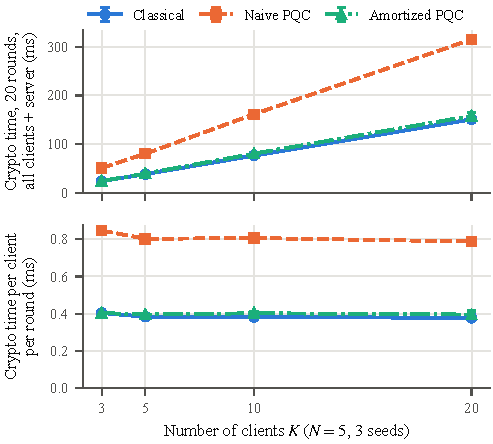
\includegraphics[width=\columnwidth]{client_scaling.pdf}
  \caption{Crypto overhead versus number of clients $K$.}
  \label{fig:scaling}
\end{figure}

% Generated by scripts/make_report_assets.py -- do not edit by hand.
% PLACEHOLDER: built from --quick profile data, not the full experiment.
\begin{table*}[t]
\centering
\footnotesize
\caption{[PLACEHOLDER: quick-profile data] Crypto cost versus number of clients $K$}
\label{tab:scaling}
\setlength{\tabcolsep}{4pt}
\begin{tabular}{lrrrrrr}
\toprule
$K$ & \multicolumn{2}{c}{Classical} & \multicolumn{2}{c}{Naive PQC} & \multicolumn{2}{c}{Amortized PQC} \\
\cmidrule(lr){2-3}\cmidrule(lr){4-5}\cmidrule(lr){6-7}
 & Crypto (ms) & \% round & Crypto (ms) & \% round & Crypto (ms) & \% round \\
\midrule
3 & 6.96 $\pm$ 0.07 & 0.818 $\pm$ 0.018 & 10.88 $\pm$ 0.27 & 1.261 $\pm$ 0.078 & 7.42 $\pm$ 0.08 & 0.883 $\pm$ 0.003 \\
5 & 10.72 $\pm$ 0.45 & 0.784 $\pm$ 0.049 & 17.40 $\pm$ 0.08 & 1.264 $\pm$ 0.015 & 11.87 $\pm$ 0.18 & 0.859 $\pm$ 0.020 \\
\bottomrule
\end{tabular}
\\[2pt]\parbox{\linewidth}{\scriptsize $N=2$ (Naive PQC: $N=1$), 4 rounds, 2 seeds; times summed over all clients and the server.}
\end{table*}


\subsection{Model Quality}

\begin{figure}[t]
  \centering
  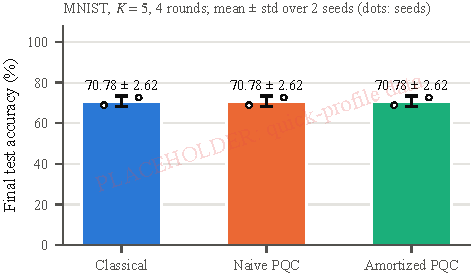
\includegraphics[width=\columnwidth]{accuracy.pdf}
  \caption{Final test accuracy per mode (mean $\pm$ std over seeds).}
  \label{fig:accuracy}
\end{figure}

% Generated by scripts/make_report_assets.py -- do not edit by hand.
% PLACEHOLDER: built from --quick profile data, not the full experiment.
\begin{table}[t]
\centering
\footnotesize
\caption{[PLACEHOLDER: quick-profile data] Final test accuracy (\%) per mode and seed}
\label{tab:accuracy}
\setlength{\tabcolsep}{4pt}
\begin{tabular}{lrrrr}
\toprule
Seed & Classical & Naive PQC & Amortized PQC & max $|\Delta|$ any round \\
\midrule
0 & 68.93 & 68.93 & 68.93 & 0.00 \\
1 & 72.63 & 72.63 & 72.63 & 0.00 \\
\midrule
Mean & 70.78 $\pm$ 2.62 & 70.78 $\pm$ 2.62 & 70.78 $\pm$ 2.62 &  \\
\bottomrule
\end{tabular}
\end{table}


\section{Security Evaluation}

% Generated by scripts/make_report_assets.py -- do not edit by hand.
\begin{table*}[t]
\centering
\footnotesize
\caption{Qualitative security comparison}
\label{tab:security}
\setlength{\tabcolsep}{4pt}
\begin{tabular}{>{\raggedright\arraybackslash}p{0.17\linewidth}>{\raggedright\arraybackslash}p{0.255\linewidth}>{\raggedright\arraybackslash}p{0.255\linewidth}>{\raggedright\arraybackslash}p{0.255\linewidth}}
\toprule
Threat & Classical ($N=5$) & Naive PQC & Amortized PQC ($N=5$) \\
\midrule
Harvest-now-decrypt-later & Not protected (X25519 secrets recoverable by a future quantum adversary)\newline{\scriptsize (no test: property of the primitive)} & Protected (ML-KEM-768)\newline{\scriptsize\texttt{wire\_\allowbreak{}sizes}} & Protected (ML-KEM-768)\newline{\scriptsize\texttt{wire\_\allowbreak{}sizes}} \\
Active MITM on the handshake & Protected$^{\dagger}$ (Ed25519, both directions)\newline{\scriptsize\texttt{forged\_\allowbreak{}server\_\allowbreak{}response\_\allowbreak{}rejected}}\newline{\scriptsize\texttt{substituted\_\allowbreak{}kem\_\allowbreak{}key\_\allowbreak{}rejected}} & Protected (ML-DSA-65, both directions)\newline{\scriptsize\texttt{forged\_\allowbreak{}server\_\allowbreak{}response\_\allowbreak{}rejected}}\newline{\scriptsize\texttt{substituted\_\allowbreak{}kem\_\allowbreak{}key\_\allowbreak{}rejected}} & Protected (ML-DSA-65, both directions)\newline{\scriptsize\texttt{forged\_\allowbreak{}server\_\allowbreak{}response\_\allowbreak{}rejected}}\newline{\scriptsize\texttt{substituted\_\allowbreak{}kem\_\allowbreak{}key\_\allowbreak{}rejected}} \\
Replayed update & Protected\newline{\scriptsize\texttt{replayed\_\allowbreak{}update\_\allowbreak{}from\_\allowbreak{}old\_\allowbreak{}round\_\allowbreak{}rejected}} & Protected\newline{\scriptsize\texttt{replayed\_\allowbreak{}update\_\allowbreak{}from\_\allowbreak{}old\_\allowbreak{}round\_\allowbreak{}rejected}} & Protected\newline{\scriptsize\texttt{replayed\_\allowbreak{}update\_\allowbreak{}from\_\allowbreak{}old\_\allowbreak{}round\_\allowbreak{}rejected}} \\
Reordered / duplicate update & Protected\newline{\scriptsize\texttt{reordered\_\allowbreak{}update\_\allowbreak{}rejected}}\newline{\scriptsize\texttt{rollback\_\allowbreak{}to\_\allowbreak{}earlier\_\allowbreak{}round\_\allowbreak{}rejected}} & Protected (future-round key does not exist yet)\newline{\scriptsize\texttt{replayed\_\allowbreak{}update\_\allowbreak{}from\_\allowbreak{}old\_\allowbreak{}round\_\allowbreak{}rejected}} & Protected\newline{\scriptsize\texttt{reordered\_\allowbreak{}update\_\allowbreak{}rejected}} \\
Tampered ciphertext & Protected\newline{\scriptsize\texttt{tampered\_\allowbreak{}ciphertext\_\allowbreak{}rejected}} & Protected\newline{\scriptsize\texttt{tampered\_\allowbreak{}ciphertext\_\allowbreak{}rejected}} & Protected\newline{\scriptsize\texttt{tampered\_\allowbreak{}ciphertext\_\allowbreak{}rejected}} \\
Session-key compromise exposure window & Bounded by $N$ rounds (whole session if keyed once)\newline{\scriptsize\texttt{old\_\allowbreak{}epoch\_\allowbreak{}key\_\allowbreak{}rejected\_\allowbreak{}after\_\allowbreak{}rekey}} & Protected beyond 1 round (fresh key every round)\newline{\scriptsize\texttt{roundtrip\_\allowbreak{}and\_\allowbreak{}rekey\_\allowbreak{}schedule}} & Bounded by $N$ rounds\newline{\scriptsize\texttt{old\_\allowbreak{}epoch\_\allowbreak{}key\_\allowbreak{}rejected\_\allowbreak{}after\_\allowbreak{}rekey}} \\
\bottomrule
\end{tabular}
\\[2pt]\parbox{\linewidth}{\scriptsize Test names refer to \texttt{tests/test\_crypto.py} (prefix \texttt{test\_} omitted). $^{\dagger}$Against classical adversaries; a quantum-capable active attacker could forge Ed25519 in real time. Exposure window: updates readable after compromise of one session key $K_e$; long-term identity-key compromise exposes no past updates in any mode (fresh KEM keys per epoch) but allows impersonation in later handshakes.}
\end{table*}


% Generated by scripts/make_report_assets.py -- do not edit by hand.
\begin{table*}[t]
\centering
\footnotesize
\caption{Automated tests (pytest); parametrized cases are counted per test}
\label{tab:tests}
\setlength{\tabcolsep}{4pt}
\begin{tabular}{>{\raggedright\arraybackslash}p{0.31\linewidth}p{0.54\linewidth}r}
\toprule
Test & Purpose & Result \\
\midrule
\multicolumn{3}{l}{\textit{Crypto layer (\texttt{tests/test\_crypto.py})}} \\
\texttt{\scriptsize roundtrip\_\allowbreak{}and\_\allowbreak{}rekey\_\allowbreak{}schedule} & Round trip over 7 rounds; handshake count follows the mode's re-key schedule & pass (4/4) \\
\texttt{\scriptsize nonces\_\allowbreak{}unique\_\allowbreak{}and\_\allowbreak{}ciphertexts\_\allowbreak{}differ} & 50 encryptions of one plaintext use 50 distinct 96-bit nonces & pass (4/4) \\
\texttt{\scriptsize partial\_\allowbreak{}participation\_\allowbreak{}late\_\allowbreak{}joiner} & Client joining late keys the epoch the schedule prescribes & pass (2/2) \\
\texttt{\scriptsize encrypt\_\allowbreak{}without\_\allowbreak{}session\_\allowbreak{}raises} & Encryption is refused before a handshake & pass (4/4) \\
\texttt{\scriptsize tampered\_\allowbreak{}ciphertext\_\allowbreak{}rejected} & Bit flips in ciphertext, tag or nonce, truncation, client-ID swap fail the AEAD & pass (20/20) \\
\texttt{\scriptsize replayed\_\allowbreak{}update\_\allowbreak{}from\_\allowbreak{}old\_\allowbreak{}round\_\allowbreak{}rejected} & Old-round update rejected verbatim, with rewritten header, and as a duplicate & pass (4/4) \\
\texttt{\scriptsize reordered\_\allowbreak{}update\_\allowbreak{}rejected} & Update for a future round is rejected & pass (3/3) \\
\texttt{\scriptsize rollback\_\allowbreak{}to\_\allowbreak{}earlier\_\allowbreak{}round\_\allowbreak{}rejected} & Fresh update for a round before the last accepted one is rejected & pass (1/1) \\
\texttt{\scriptsize old\_\allowbreak{}epoch\_\allowbreak{}key\_\allowbreak{}rejected\_\allowbreak{}after\_\allowbreak{}rekey} & Update under the pre-re-key session key is rejected & pass (2/2) \\
\texttt{\scriptsize update\_\allowbreak{}with\_\allowbreak{}wrong\_\allowbreak{}epoch\_\allowbreak{}header\_\allowbreak{}rejected} & Update whose header epoch disagrees with the schedule is rejected & pass (2/2) \\
\texttt{\scriptsize server\_\allowbreak{}rejects\_\allowbreak{}update\_\allowbreak{}when\_\allowbreak{}client\_\allowbreak{}skipped\_\allowbreak{}rekey} & Client that skipped a scheduled re-key is rejected & pass (2/2) \\
\texttt{\scriptsize handshake\_\allowbreak{}for\_\allowbreak{}wrong\_\allowbreak{}epoch\_\allowbreak{}rejected} & Handshake signed for a different epoch is rejected & pass (2/2) \\
\texttt{\scriptsize replayed\_\allowbreak{}handshake\_\allowbreak{}rejected} & Replayed old handshake cannot overwrite a live session & pass (2/2) \\
\texttt{\scriptsize impostor\_\allowbreak{}signing\_\allowbreak{}with\_\allowbreak{}own\_\allowbreak{}key\_\allowbreak{}rejected} & Handshake signed with a key not registered for the claimed ID is rejected & pass (4/4) \\
\texttt{\scriptsize bitflipped\_\allowbreak{}signature\_\allowbreak{}rejected} & Corrupted or empty client signatures are rejected & pass (4/4) \\
\texttt{\scriptsize substituted\_\allowbreak{}kem\_\allowbreak{}key\_\allowbreak{}rejected} & MITM substitution of the client's KEM public key is rejected & pass (4/4) \\
\texttt{\scriptsize signature\_\allowbreak{}does\_\allowbreak{}not\_\allowbreak{}transfer\_\allowbreak{}across\_\allowbreak{}epochs} & A signature from one epoch cannot authorize another & pass (2/2) \\
\texttt{\scriptsize unknown\_\allowbreak{}client\_\allowbreak{}rejected} & Handshake from an unregistered client ID is rejected & pass (4/4) \\
\texttt{\scriptsize forged\_\allowbreak{}server\_\allowbreak{}response\_\allowbreak{}rejected} & Client rejects a MITM re-encapsulated or re-signed server response & pass (4/4) \\
\texttt{\scriptsize invalid\_\allowbreak{}config\_\allowbreak{}rejected} & Invalid mode / re-key interval combinations are rejected & pass (4/4) \\
\texttt{\scriptsize config\_\allowbreak{}accepts\_\allowbreak{}mode\_\allowbreak{}strings} & Modes can be given as strings; naive PQC fixes $N=1$ & pass (1/1) \\
\texttt{\scriptsize classical\_\allowbreak{}rekey\_\allowbreak{}interval\_\allowbreak{}accepted} & Classical mode accepts key-once or a re-key interval & pass (1/1) \\
\texttt{\scriptsize server\_\allowbreak{}signs\_\allowbreak{}response\_\allowbreak{}in\_\allowbreak{}every\_\allowbreak{}mode} & Server response is signed (Ed25519 / ML-DSA-65) in every mode & pass (4/4) \\
\texttt{\scriptsize wire\_\allowbreak{}sizes} & Key, ciphertext and signature sizes match FIPS 203/204; 16-byte GCM tag & pass (1/1) \\
\midrule
\multicolumn{3}{l}{\textit{FL harness (\texttt{tests/test\_fl.py})}} \\
\texttt{\scriptsize flat\_\allowbreak{}params\_\allowbreak{}roundtrip} & Model parameters survive flatten / restore; size mismatch is rejected & pass (1/1) \\
\texttt{\scriptsize update\_\allowbreak{}serialization\_\allowbreak{}roundtrip\_\allowbreak{}and\_\allowbreak{}validation} & Update (de)serialization round trip; wrong size, truncation, NaN rejected & pass (1/1) \\
\texttt{\scriptsize fedavg\_\allowbreak{}is\_\allowbreak{}sample\_\allowbreak{}weighted} & FedAvg computes the sample-weighted mean & pass (1/1) \\
\texttt{\scriptsize splits\_\allowbreak{}partition\_\allowbreak{}the\_\allowbreak{}data} & IID and Dirichlet splits are disjoint and cover the dataset & pass (2/2) \\
\texttt{\scriptsize metered\_\allowbreak{}suite\_\allowbreak{}times\_\allowbreak{}ops\_\allowbreak{}and\_\allowbreak{}interoperates} & Instrumented suite times each primitive and derives identical keys & pass (1/1) \\
\texttt{\scriptsize harness\_\allowbreak{}rekey\_\allowbreak{}schedule\_\allowbreak{}and\_\allowbreak{}csv} & Harness handshake schedule, CSV schema and per-component byte counts & pass (4/4) \\
\texttt{\scriptsize harness\_\allowbreak{}is\_\allowbreak{}deterministic\_\allowbreak{}and\_\allowbreak{}mode\_\allowbreak{}independent} & Same seed gives identical accuracy in every mode & pass (1/1) \\
\texttt{\scriptsize harness\_\allowbreak{}drops\_\allowbreak{}tampered\_\allowbreak{}and\_\allowbreak{}replayed\_\allowbreak{}updates} & Tampered and replayed updates are excluded from aggregation & pass (1/1) \\
\texttt{\scriptsize harness\_\allowbreak{}keeps\_\allowbreak{}global\_\allowbreak{}model\_\allowbreak{}when\_\allowbreak{}all\_\allowbreak{}updates\_\allowbreak{}rejected} & If every update is rejected the global model is unchanged & pass (1/1) \\
\bottomrule
\end{tabular}
\\[2pt]\parbox{\linewidth}{\scriptsize 98/98 test cases passed.}
\end{table*}


\section{Discussion and Limitations}

\section{Related Work}

\section{Conclusion}

% \bibliographystyle{IEEEtran}
% \bibliography{refs}

\appendices
\section{Implementation Notes}
% Issues hit during the build and their fixes (bullet list; mirrors build_issues.md).
\begin{itemize}
  \item \textbf{KEM input lengths unchecked by liboqs-python.} \texttt{encap\_secret()} accepted a 1,183-byte ML-KEM-768 public key (expected 1,184) without error. \emph{Fix:} wrapper validates public-key and ciphertext lengths; malformed keys are rejected as authentication failures.
  \item \textbf{MITM on the client-only-signed handshake.} An unauthenticated KEM ciphertext let an attacker re-encapsulate and learn the client's session key. \emph{Fix:} server signs its response, bound to $H(\mathit{init})$, in every mode.
  \item \textbf{Header epoch not covered by the AEAD.} With server-side AAD, a changed header epoch still authenticates; mutation M5 showed the explicit header check is the only defense. \emph{Fix:} check retained and tested.
  \item \textbf{Cold-start timing bias.} First X25519 keygen $\approx$3.8\,ms vs.\ $\approx$31\,\textmu s warm (lazy OpenSSL init) inflated classical round~0 (8.8 vs.\ 4.0\,ms). \emph{Fix:} untimed warm-up of all primitives before round~0.
  \item \textbf{Participation-dependent epochs.} Counting handshakes would desynchronize clients that skip rounds. \emph{Fix:} scheduled epoch $e=\lfloor r/N \rfloor$; stale or non-increasing handshake epochs rejected.
  \item \textbf{Cadence-confounded baseline.} Classical originally keyed once. \emph{Fix:} classical supports the same $N$, isolating the primitives.
  \item \textbf{Training cost.} A full MNIST pass took $\approx$13\,s per round (about 9\,h for the grid). \emph{Fix:} per-client sample cap (2,000) and a run cache shared across experiments (80 distinct runs instead of 105).
  \item \textbf{Library/binding version coupling.} liboqs and liboqs-python must share major.minor; a missing library triggers a source build. \emph{Fix:} liboqs 0.16.0 (Homebrew) with liboqs-python 0.16.0.1 pinned.
  \item \textbf{Interpreter choice.} System default Python 3.14. \emph{Fix:} virtualenv on Python 3.11 for torch/torchvision wheel availability.
  \item \textbf{Manifest recorded CLI flags, not effective settings.} \emph{Fix:} effective seeds, rounds, $K$, $N$, sweeps and sample cap stored and consumed by the asset builder.
  \item \textbf{Output naming.} Naive PQC CSVs were labelled $N{=}$none. \emph{Fix:} names use the effective interval.
  \item \textbf{Benchmark conditions.} Laptop on battery at run time. \emph{Fix:} full run deferred to AC power; runs executed sequentially.
  \item \textbf{No TeX toolchain.} \emph{Fix:} \texttt{tectonic} installed for diagrams and the skeleton.
\end{itemize}


\end{document}
